% Define colors
\definecolor{arrow1}{HTML}{DB10E9} % pink
\definecolor{arrow1back}{HTML}{AA0000} % red
\definecolor{arrow2}{HTML}{000080} % blue
\definecolor{arrow2back}{HTML}{007700} % cyan
\definecolor{arrow3}{HTML}{FF8E00} % orange
\definecolor{arrow3back}{HTML}{EEBE00} % yellow
\definecolor{arrow4}{HTML}{2DCF2D} % mint / light green
\definecolor{arrow4back}{HTML}{007700} % green

\begin{SCfigure}[1.5][htbp]
    \centering
    \makebox[0.33\textwidth][c]{
        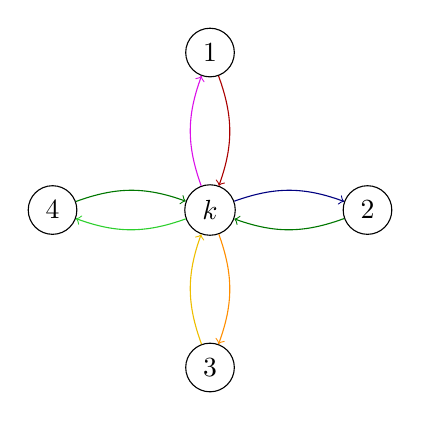
\begin{tikzpicture}
            % Central node
            \node[circle, draw, fill=white, minimum size=0.6cm] (center) at (0,0) {$k$};
        
            % Surrounding nodes
            \node[circle, draw, fill=white, minimum size=0.6cm] (n1) at (0,2) {1};
            \node[circle, draw, fill=white, minimum size=0.6cm] (n2) at (2,0) {2};
            \node[circle, draw, fill=white, minimum size=0.6cm] (n3) at (0,-2) {3};
            \node[circle, draw, fill=white, minimum size=0.6cm] (n4) at (-2,0) {4};
            
            % Arrows
            \draw[->, color=arrow1, bend left=20] (center) to (n1); % Center to 1
            \draw[<-, color=arrow1back, bend right=20] (center) to (n1); % 1 to Center

            \draw[->, color=arrow2, bend left=20] (center) to (n2); % Center to 2
            \draw[<-, color=arrow2back, bend right=20] (center) to (n2); % 2 to Center

            \draw[->, color=arrow3, bend left=20] (center) to (n3); % Center to 3
            \draw[<-, color=arrow3back, bend right=20] (center) to (n3); % 3 to Center

            \draw[->, color=arrow4, bend left=20] (center) to (n4); % Center to 4
            \draw[<-, color=arrow4back, bend right=20] (center) to (n4); % 4 to Center
            
        \end{tikzpicture}
    }
    \caption{Exemplary cutout of a square lattice. The nearest neighbors to a central node with index $k$ are depicted. The numeration is arbitrary, but matches the indices that are used in \autoref{eq:current-geometry-example}.
    The colors match the terms that correspond to their transition.
    }
    \label{fig:current-geometry-example}
\end{SCfigure}

\begin{equation}
    \label{eq:current-geometry-example}
    \begin{split}
        \partial_\text{x}
        j_{\text{x}\,\,k,\,\sigma}^{\,\,\schroedingerPicture}+
        \partial_\text{y} 
        j_{\text{y}\,\,k,\,\sigma}^{\,\,\schroedingerPicture} 
        &\stackrel{\phantom{\ref{eq:continuity-equation}}}{=}
        \textcolor{arrow2}{
            \spinPolarizedKineticsOperatorDir{k}{2}{\sigma}
        }
        -
        \textcolor{arrow4back}{
            \spinPolarizedKineticsOperatorDir{4}{k}{\sigma}
        }\\
        &\stackrel{\phantom{\ref{eq:continuity-equation}}}{+}
        \textcolor{arrow3}{
            \spinPolarizedKineticsOperatorDir{k}{3}{\sigma}
        }
        -
        \textcolor{arrow1back}{
            \spinPolarizedKineticsOperatorDir{1}{k}{\sigma}
        }\\
        & \stackrel{\ref{eq:continuity-equation}}{=}
         - i \cdot \left[\pictureHamiltonian[\schroedingerPicture],\, \nop[\schroedingerPicture]{k}{\sigma}\right]
         \stackrel{\ref{eq:calculation-current-commutator}}{=}\\
         & \hspace{-3cm} i\cdot J \left(
            \textcolor{arrow2}{
                \withspinhcop[\schroedingerPicture]{2}{\sigma}{\dagger}
                \withspinhcop[\schroedingerPicture]{k}{\sigma}{}
            }
            -
            \textcolor{arrow2back}{
                \withspinhcop[\schroedingerPicture]{k}{\sigma}{\dagger}
                \withspinhcop[\schroedingerPicture]{2}{\sigma}{}
            }
            -
            \textcolor{arrow4back}{
                \withspinhcop[\schroedingerPicture]{k}{\sigma}{\dagger}
                \withspinhcop[\schroedingerPicture]{4}{\sigma}{}
            }
            +
            \textcolor{arrow4}{
                \withspinhcop[\schroedingerPicture]{4}{\sigma}{\dagger}
                \withspinhcop[\schroedingerPicture]{k}{\sigma}{}
            }
            +
            \textcolor{arrow3}{
                \withspinhcop[\schroedingerPicture]{3}{\sigma}{\dagger}
                \withspinhcop[\schroedingerPicture]{k}{\sigma}{}
            }
            -
            \textcolor{arrow3back}{
                \withspinhcop[\schroedingerPicture]{k}{\sigma}{\dagger}
                \withspinhcop[\schroedingerPicture]{3}{\sigma}{}
            }
            -
            \textcolor{arrow1back}{
                \withspinhcop[\schroedingerPicture]{k}{\sigma}{\dagger}
                \withspinhcop[\schroedingerPicture]{1}{\sigma}{}
            }
            +
            \textcolor{arrow1}{
                \withspinhcop[\schroedingerPicture]{1}{\sigma}{\dagger}
                \withspinhcop[\schroedingerPicture]{k}{\sigma}{}
            }
         \right)
    \end{split}
\end{equation}
